\section{Results}

\subsection{Equilibrium Verification}

We verified equilibrium behavior by measuring $\langle E(T) \rangle$ and $\langle m(T) \rangle$ at our largest lattice size $L = 128$. The curves reproduce the expected ferromagnetic ordering at low $T$ and disordered phase at high $T$, with susceptibility peaks near $T_c$. This validates our simulation settings used for the dynamical analysis.

\begin{figure}[h!]
    \centering
    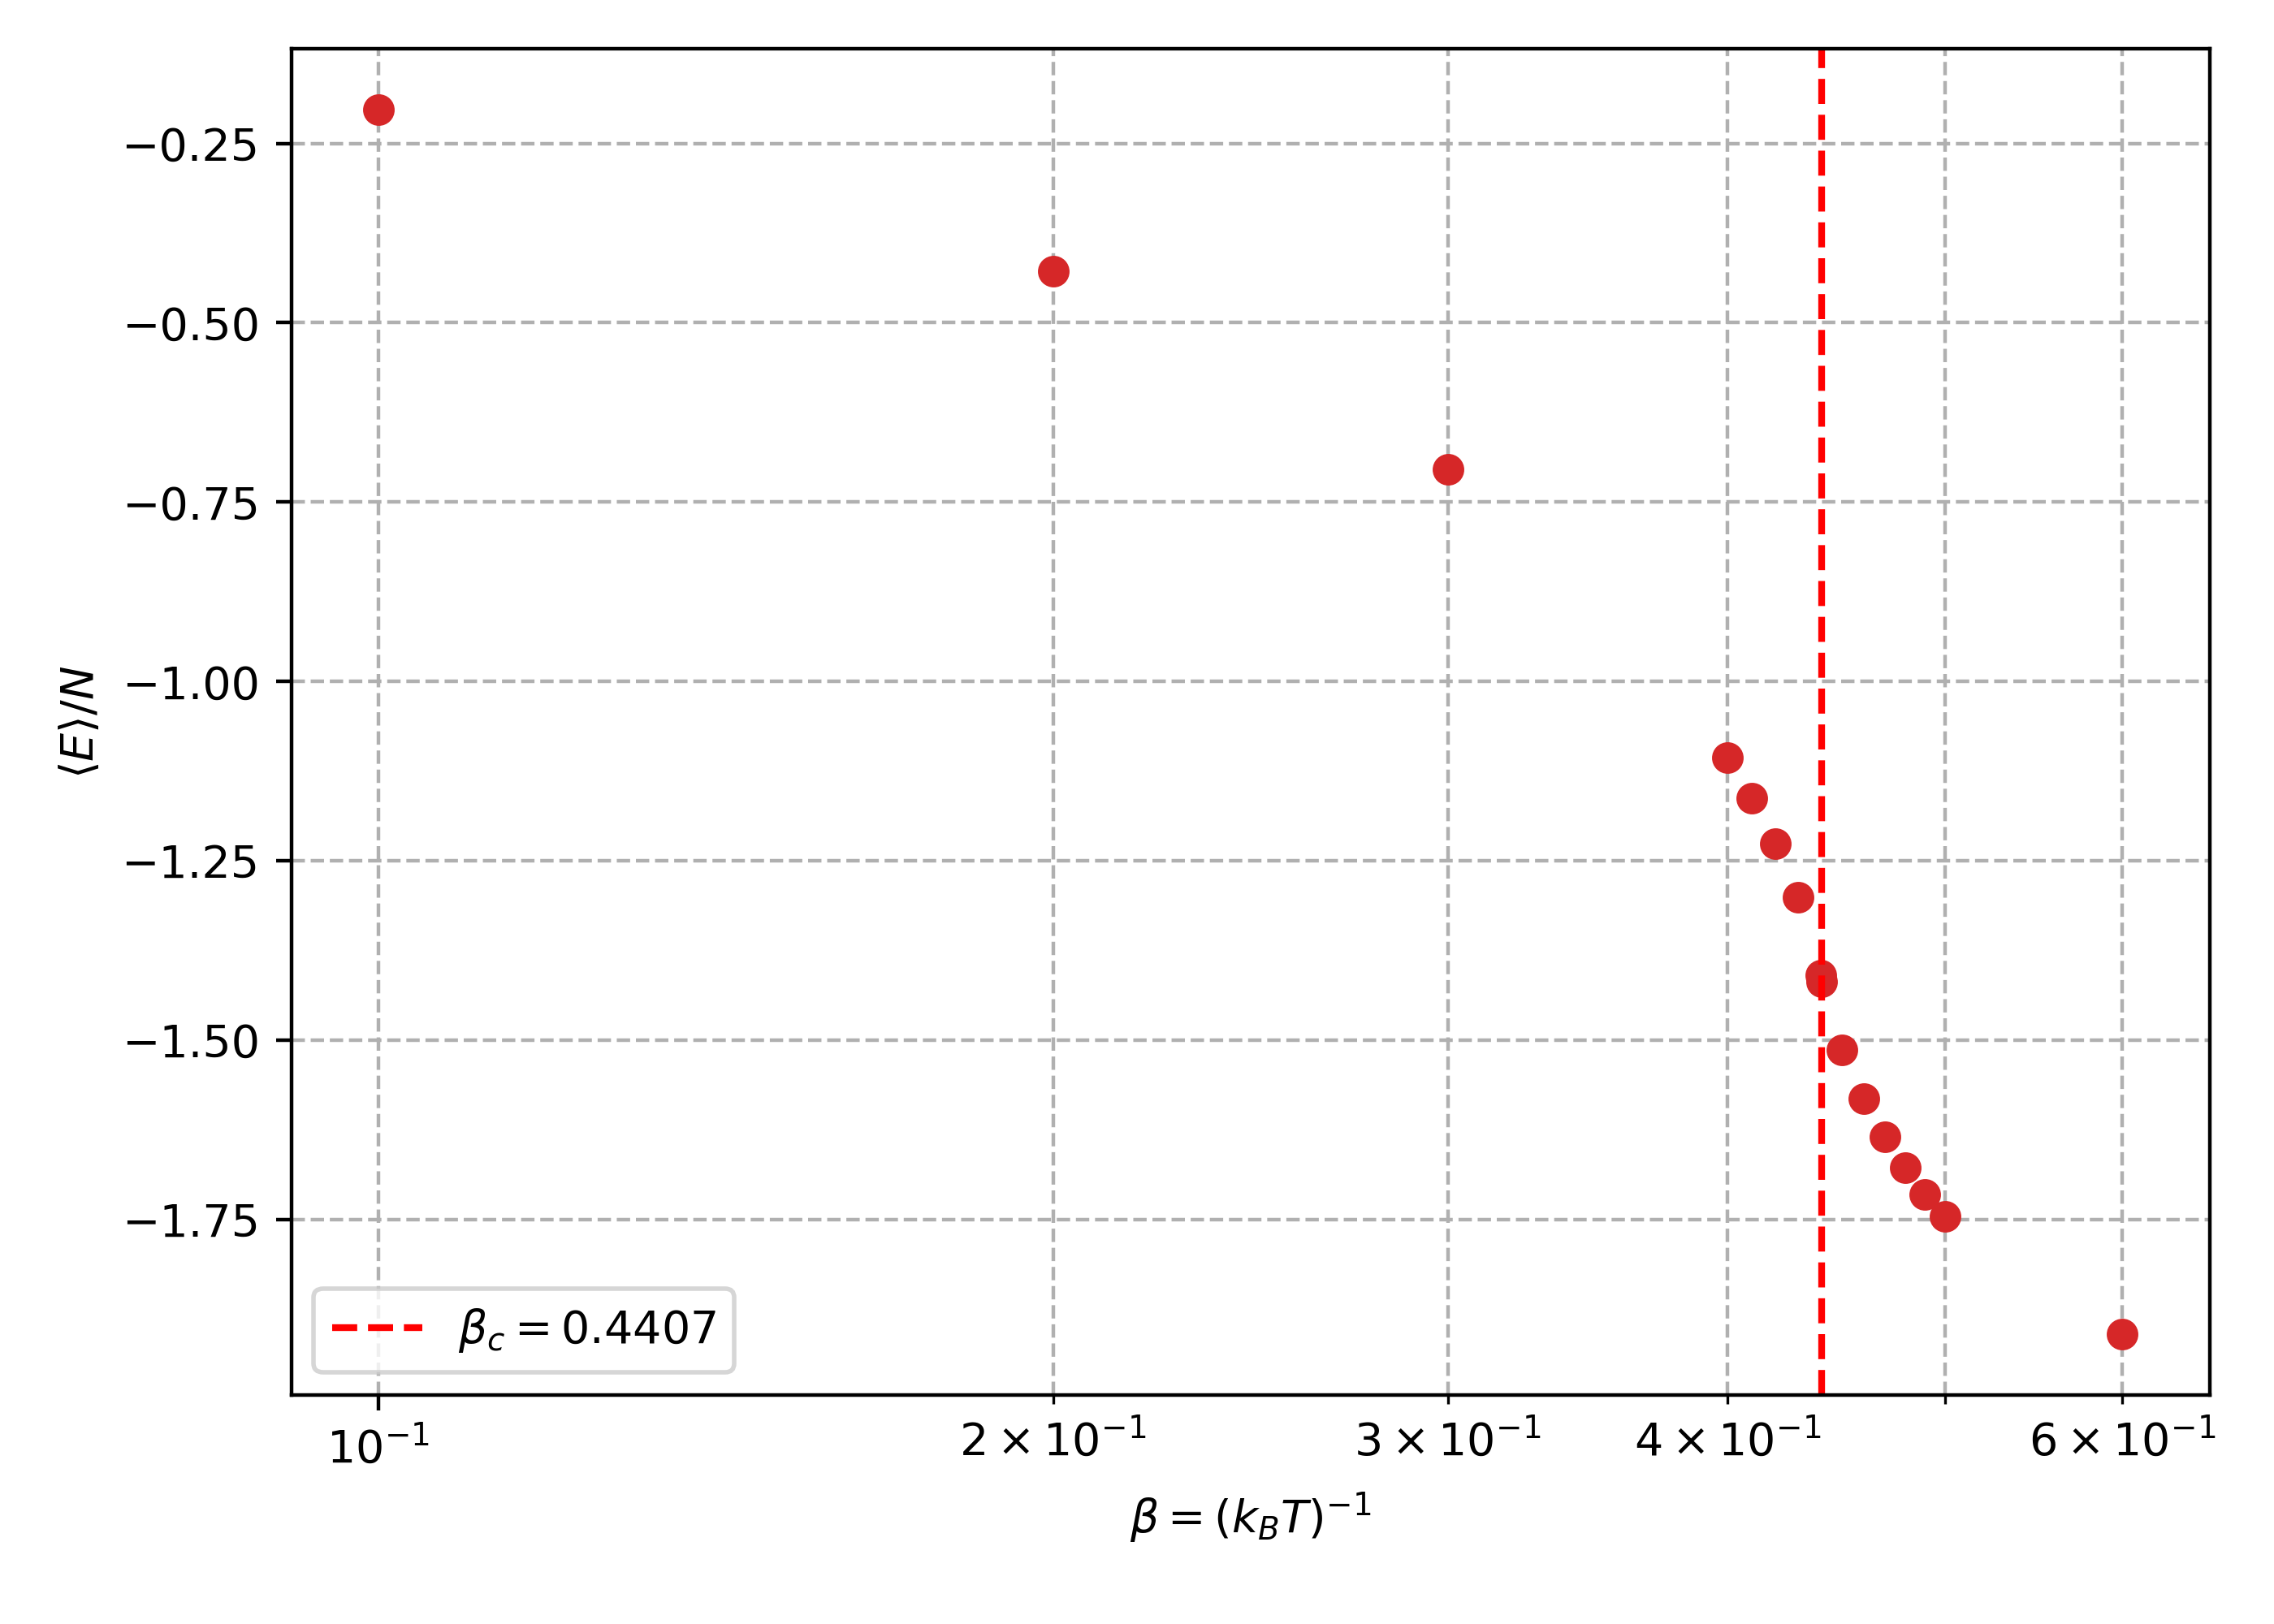
\includegraphics[width = 0.6 \textwidth]{../plots/metropolis_energy_vs_beta_xlog.png}
    \caption[Energy per spin versus $\beta$ using Metropolis updates]{Energy per spin versus $\frac{\langle E \rangle}{N}$ inverse temperature $\beta$ for the 2D Ising model using Metropolis updates. Points show the equilibrium average energy.}
\end{figure}

\begin{figure}[h!]
    \centering
    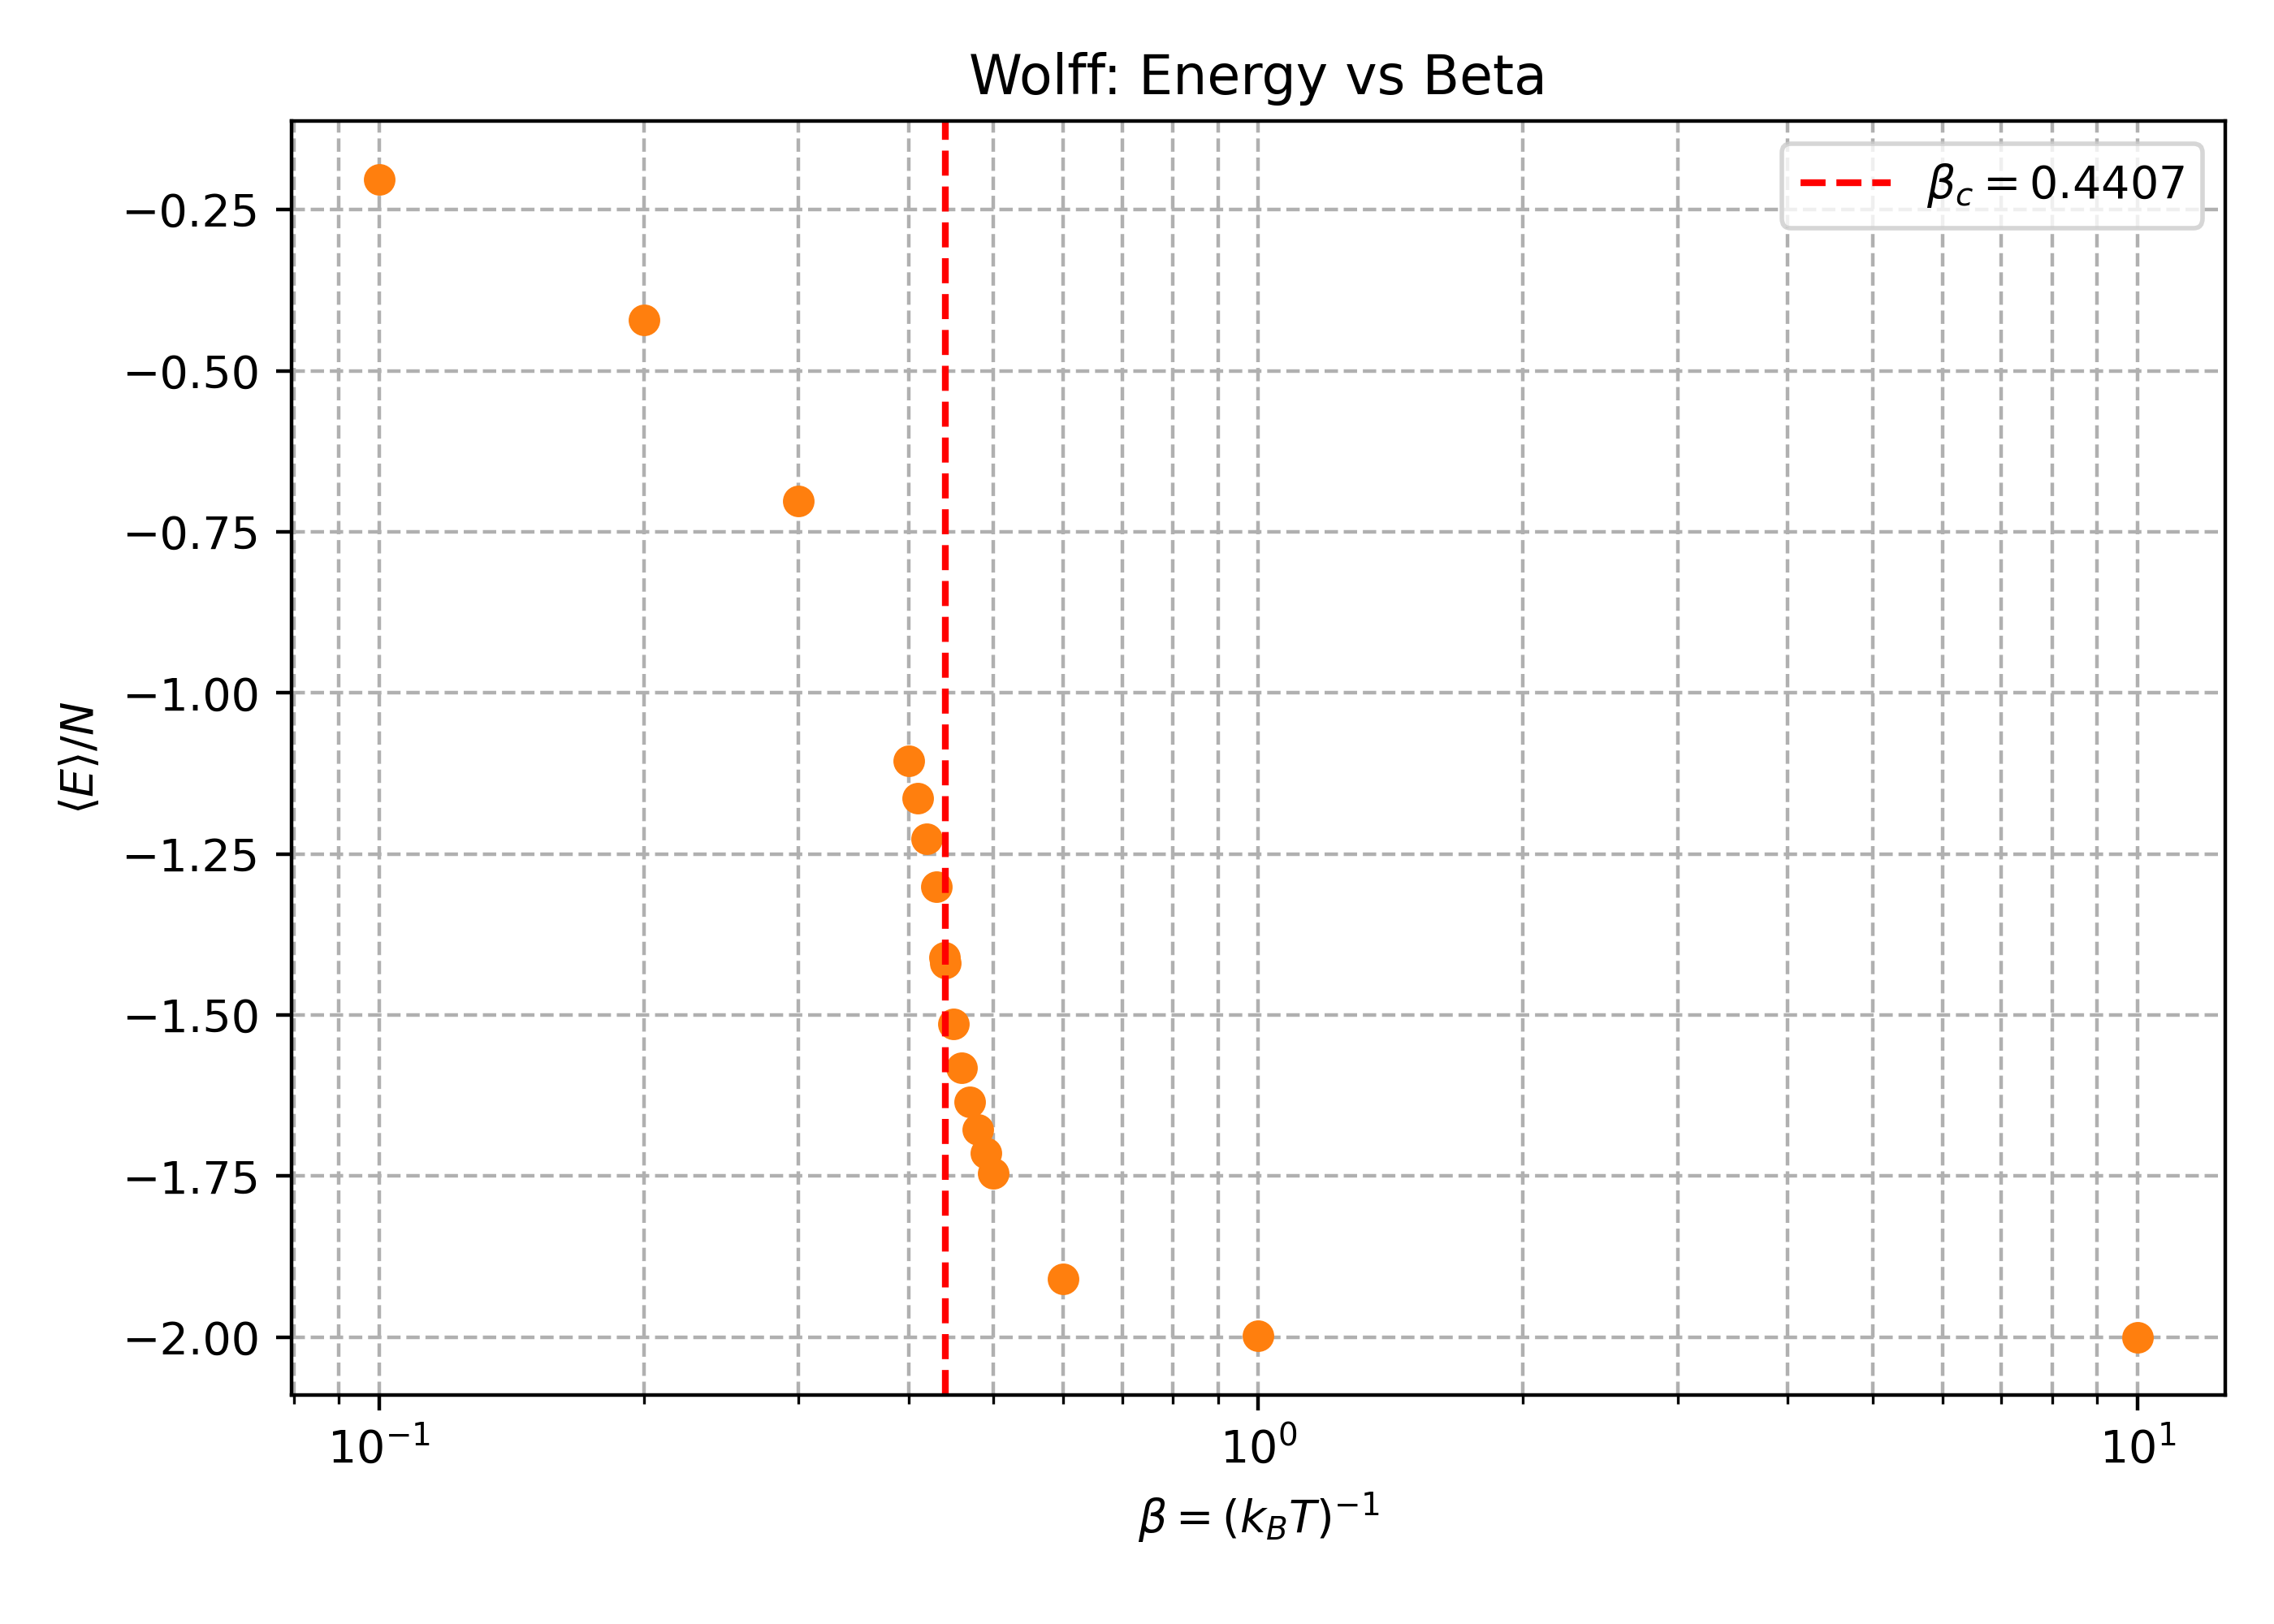
\includegraphics[width = 0.6 \textwidth]{../plots/wolff_energy_vs_beta_xlog.png}
    \caption[Energy per spin versus $\beta$ using Wolff updates]{Energy per spin versus $\frac{\langle E \rangle}{N}$ inverse temperature $\beta$ for the 2D Ising model using Wolff updates. Points show the equilibrium average energy.}
\end{figure}

We can see that for both algorithms, as $\beta$ increases, $\frac{\langle E \rangle}{N}$ decreases smoothly and exhibits a pronounced change in slope near the critical $\beta_c \approx 0.4407$ (vertical reference line).

\begin{figure}[h!]
    \centering
    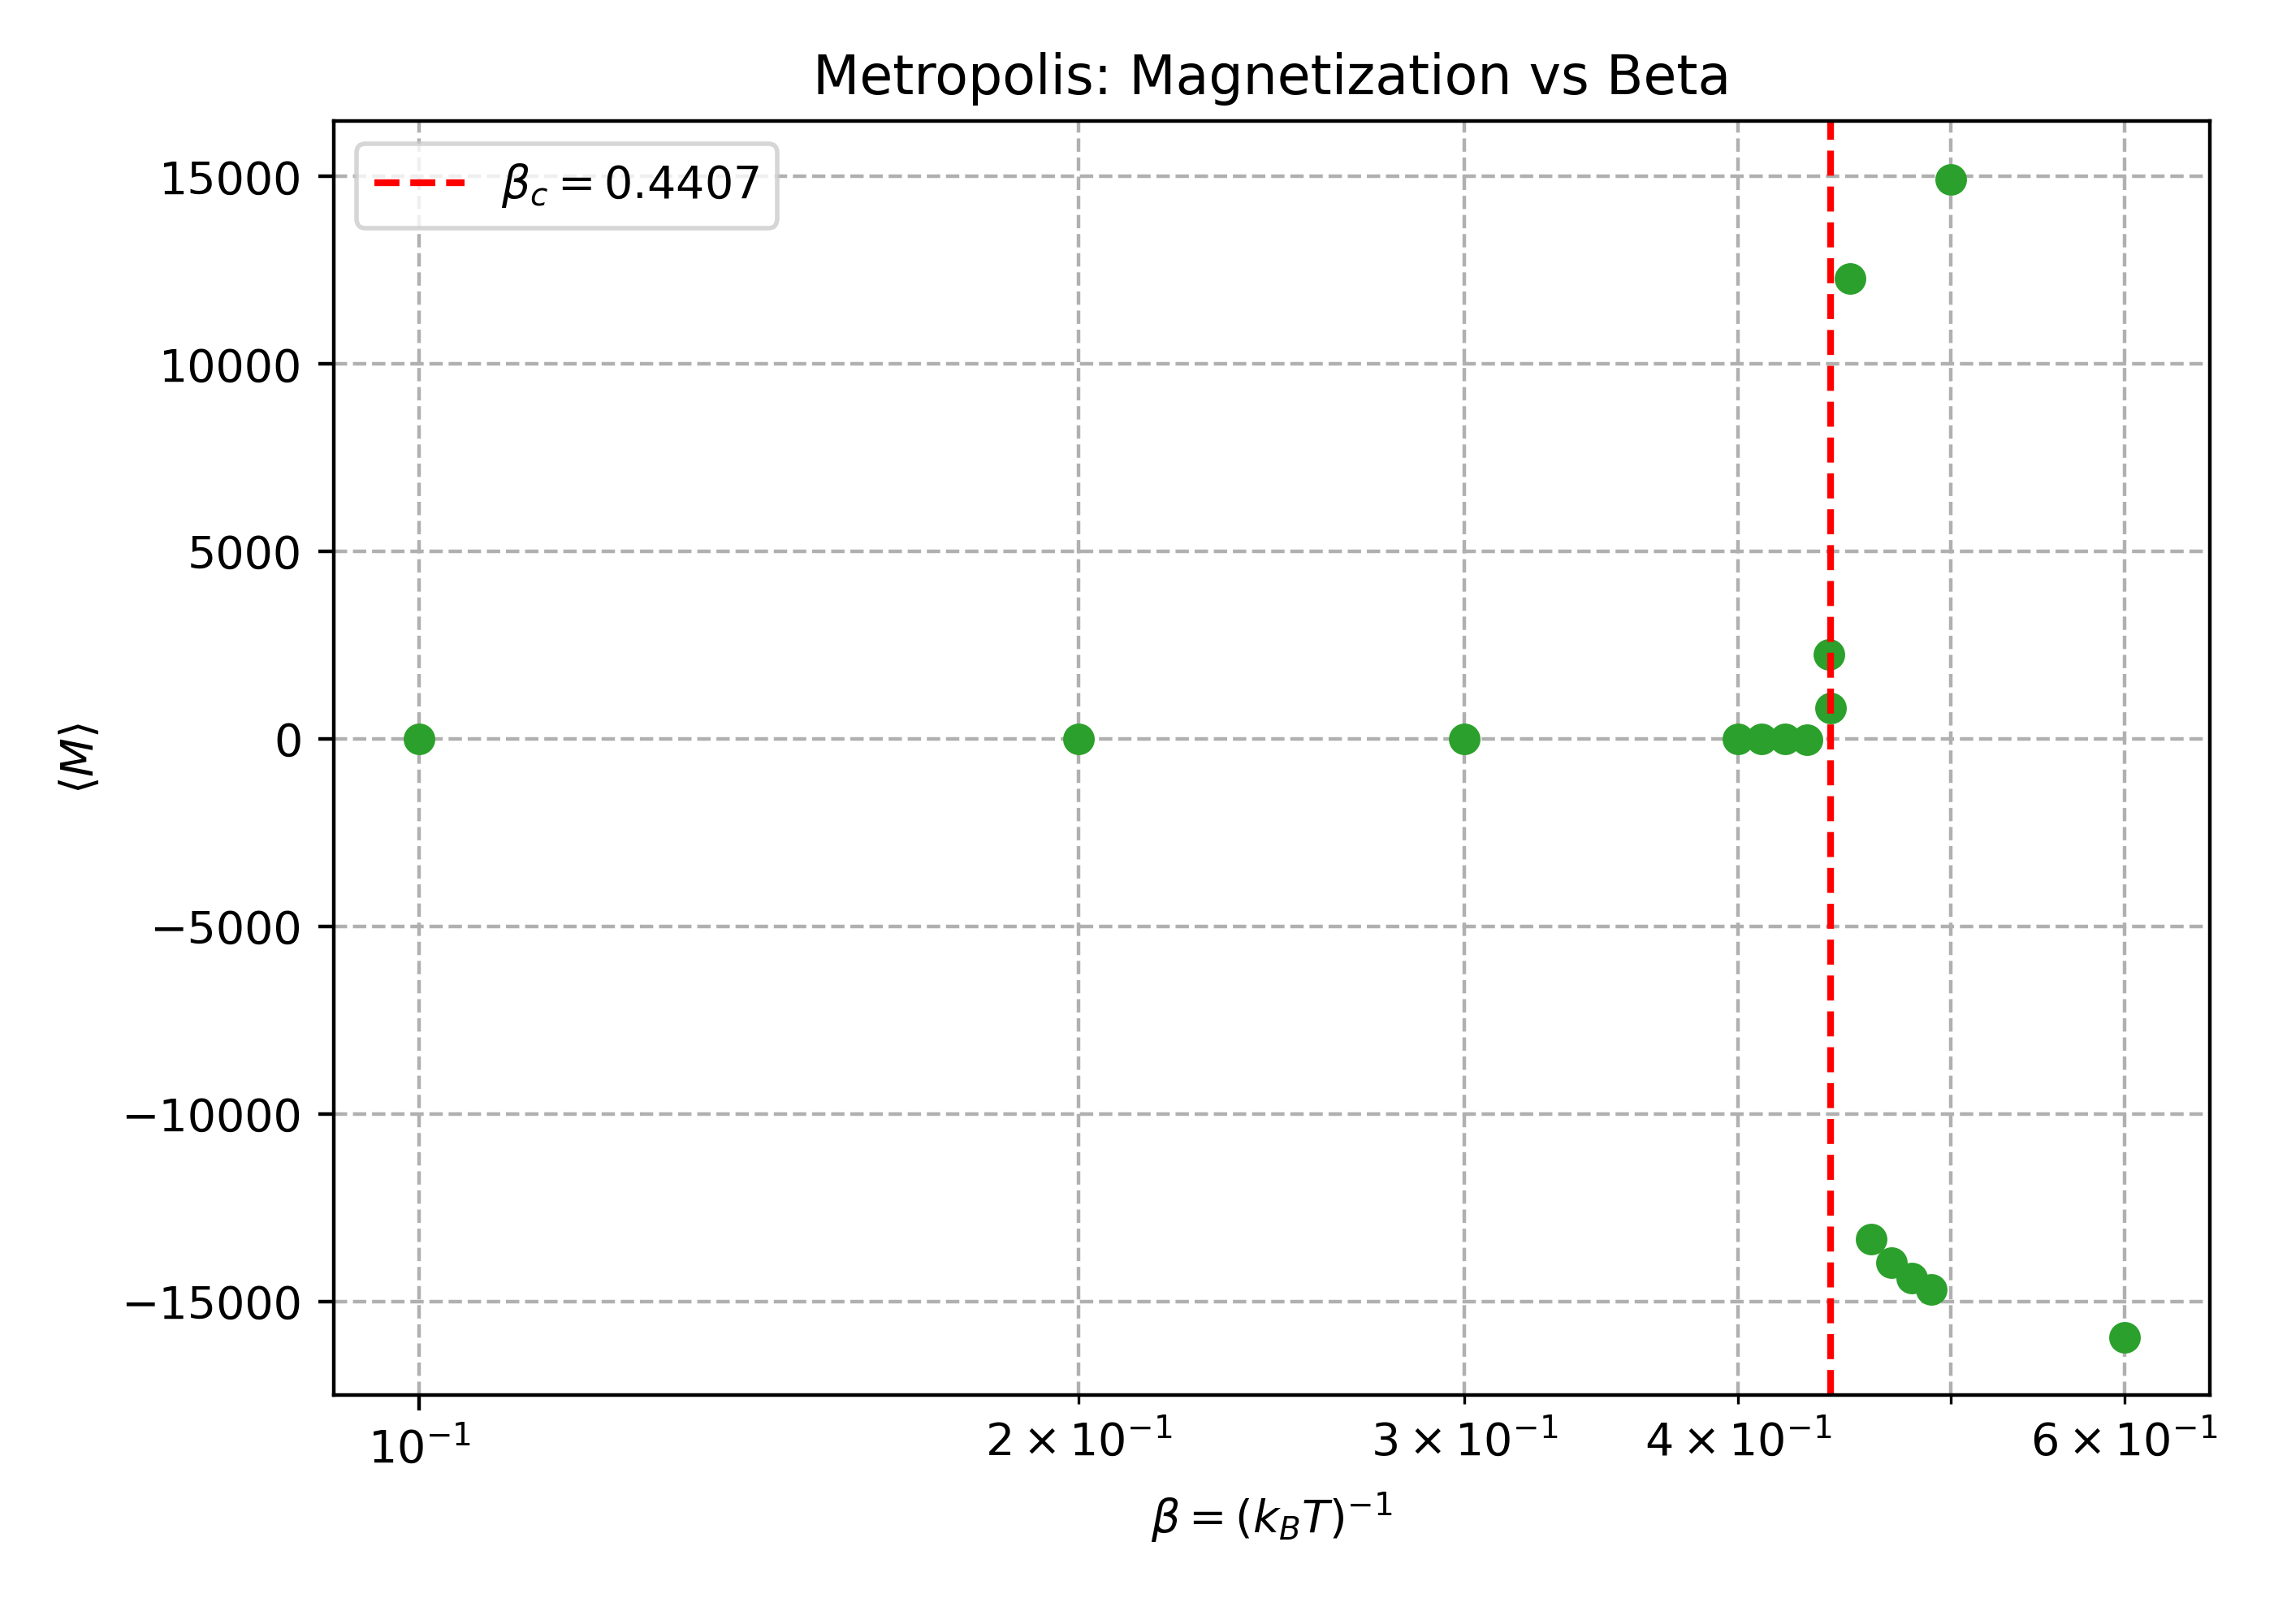
\includegraphics[width = 0.6 \textwidth]{../plots/metropolis_mag_vs_beta_xlog.png}
    \caption[Magnetization versus $\beta$ using Metropolis updates]{Magnetization versus inverse temperature $\beta$ using Metropolis updates. Points show the equilibrium average magnetization.}
\end{figure}

\begin{figure}[h!]
    \centering
    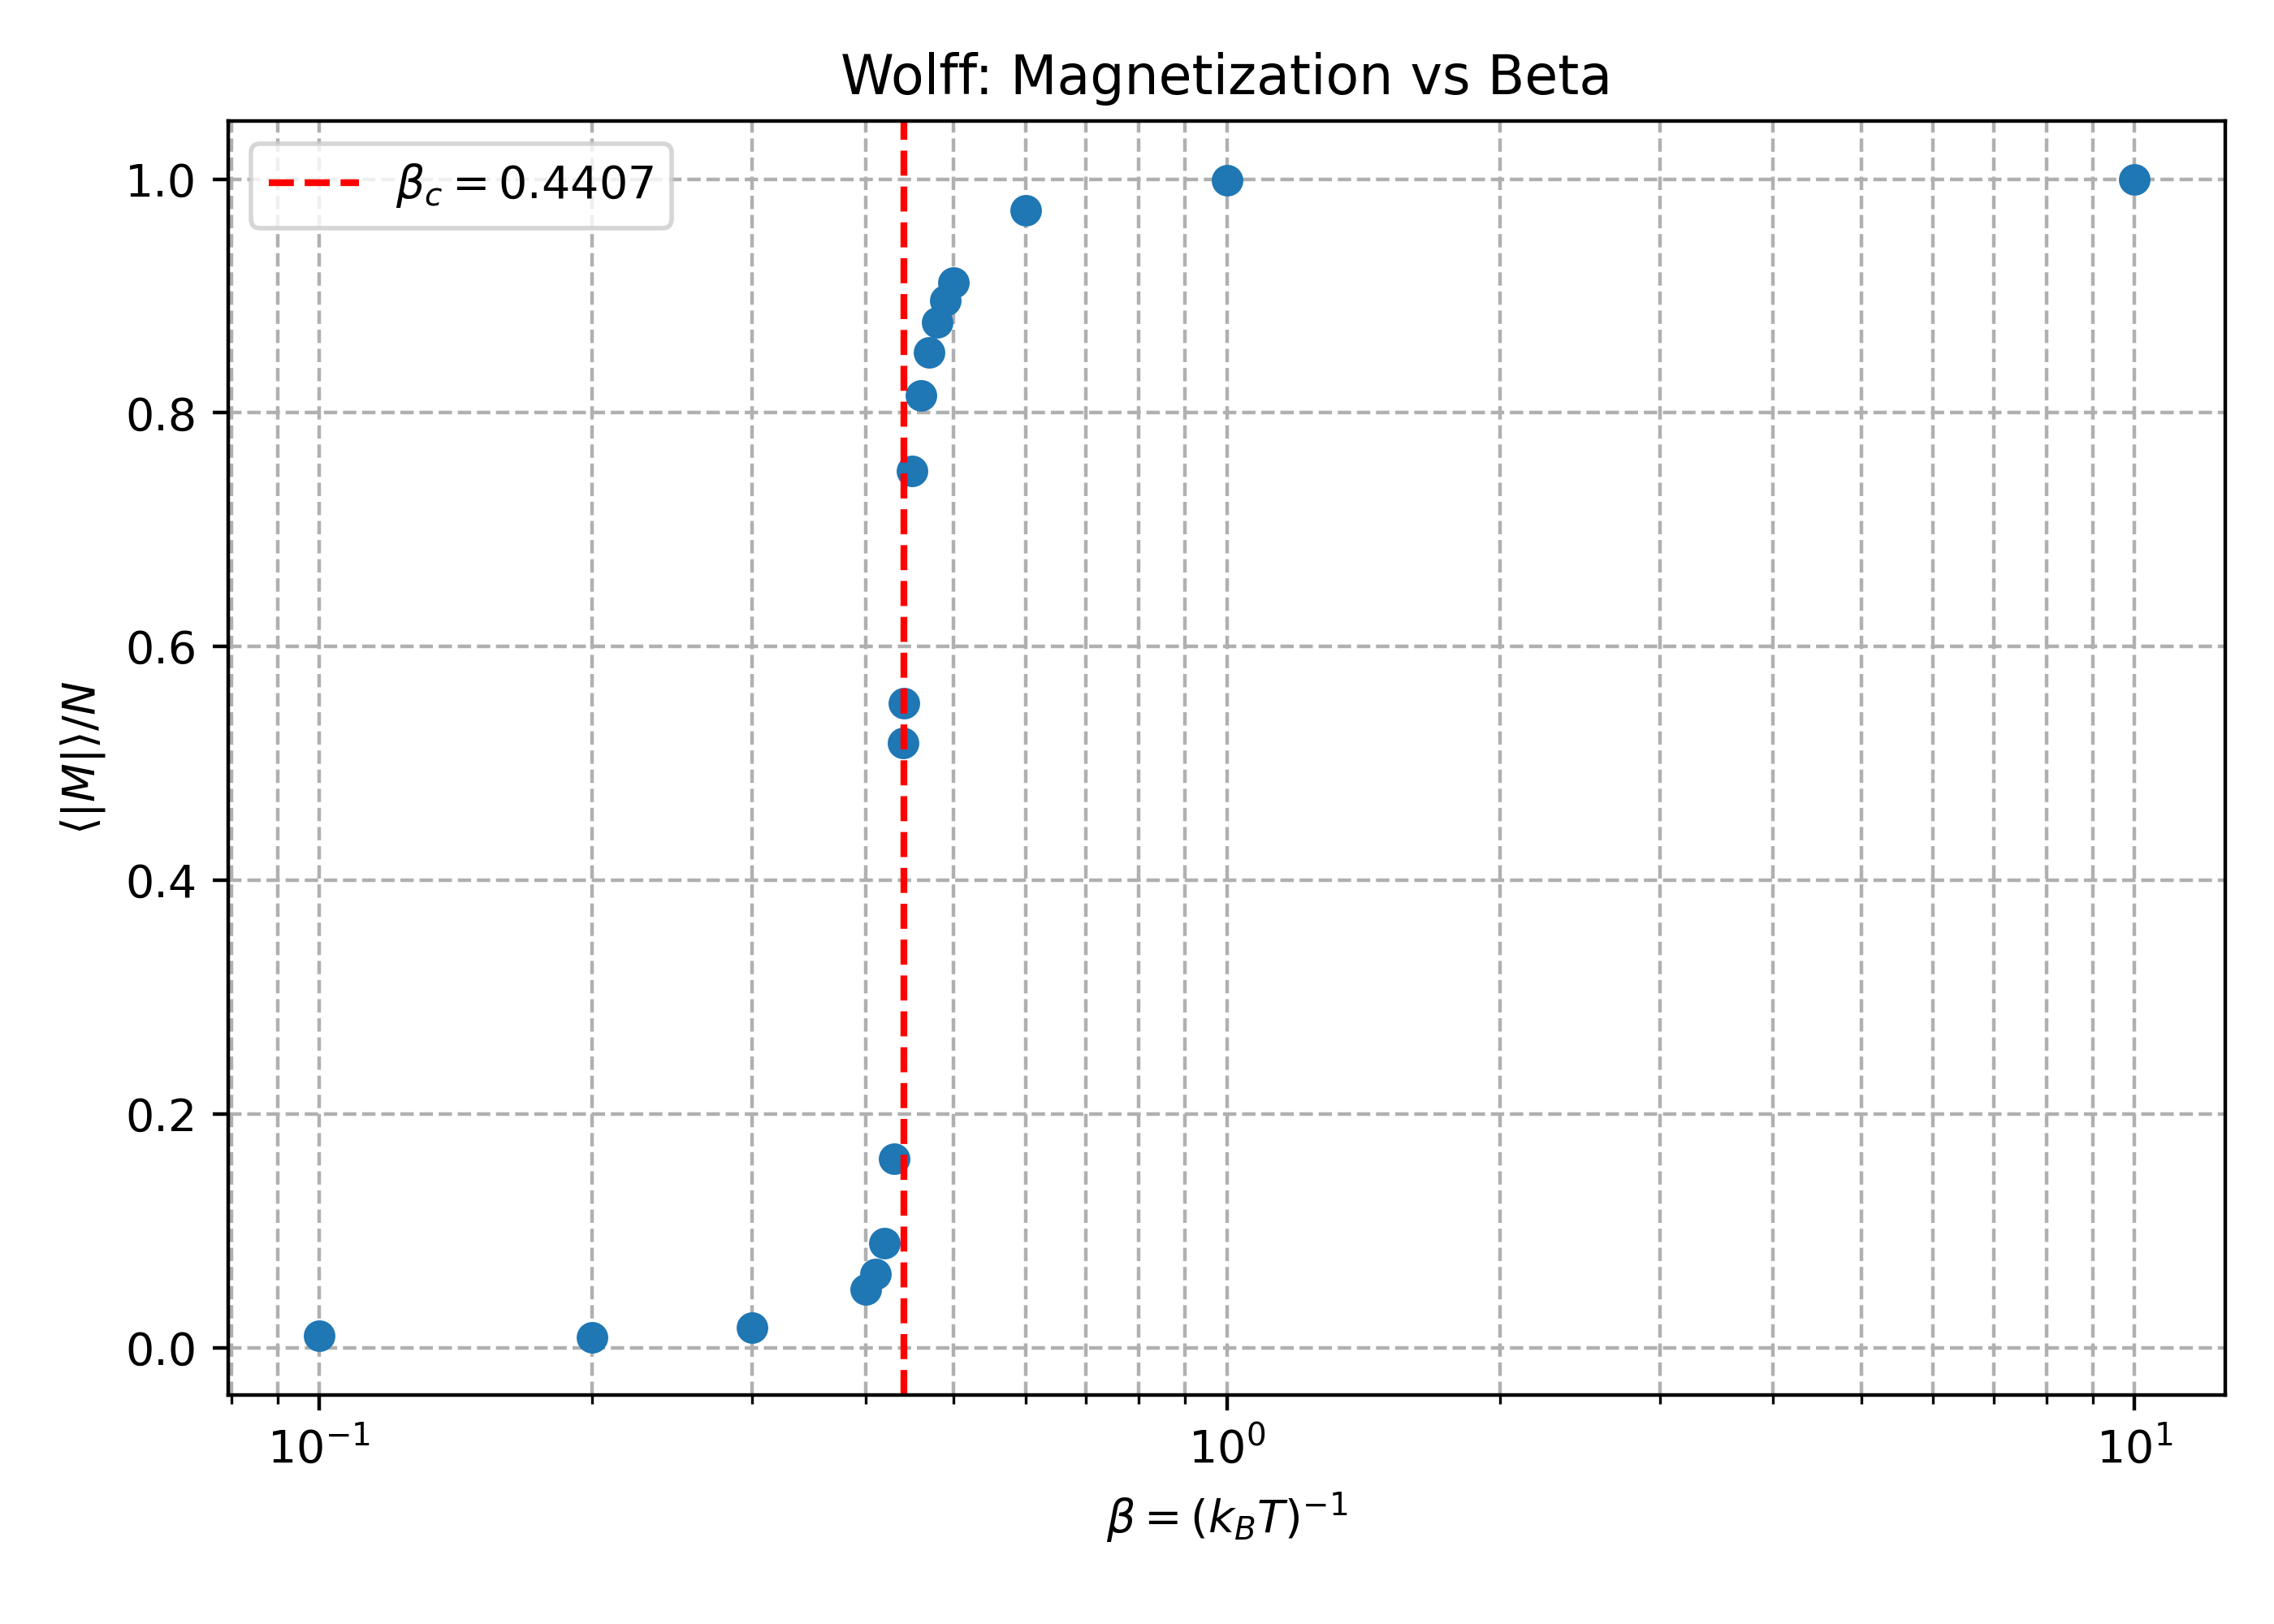
\includegraphics[width = 0.6 \textwidth]{../plots/wolff_mag_vs_beta_xlog.png}
    \caption[Magnetization versus $\beta$ using Wolff updates]{Magnetization versus inverse temperature $\beta$ using Wolff updates. Points show the equilibrium average magnetization.}
\end{figure}

Magnetization plots show the expected spontaneous magnetization below $T_c$ and decay to zero above $T_c$ for both algorithms, confirming correct equilibrium sampling.

\begin{figure}[h!]
    \centering
    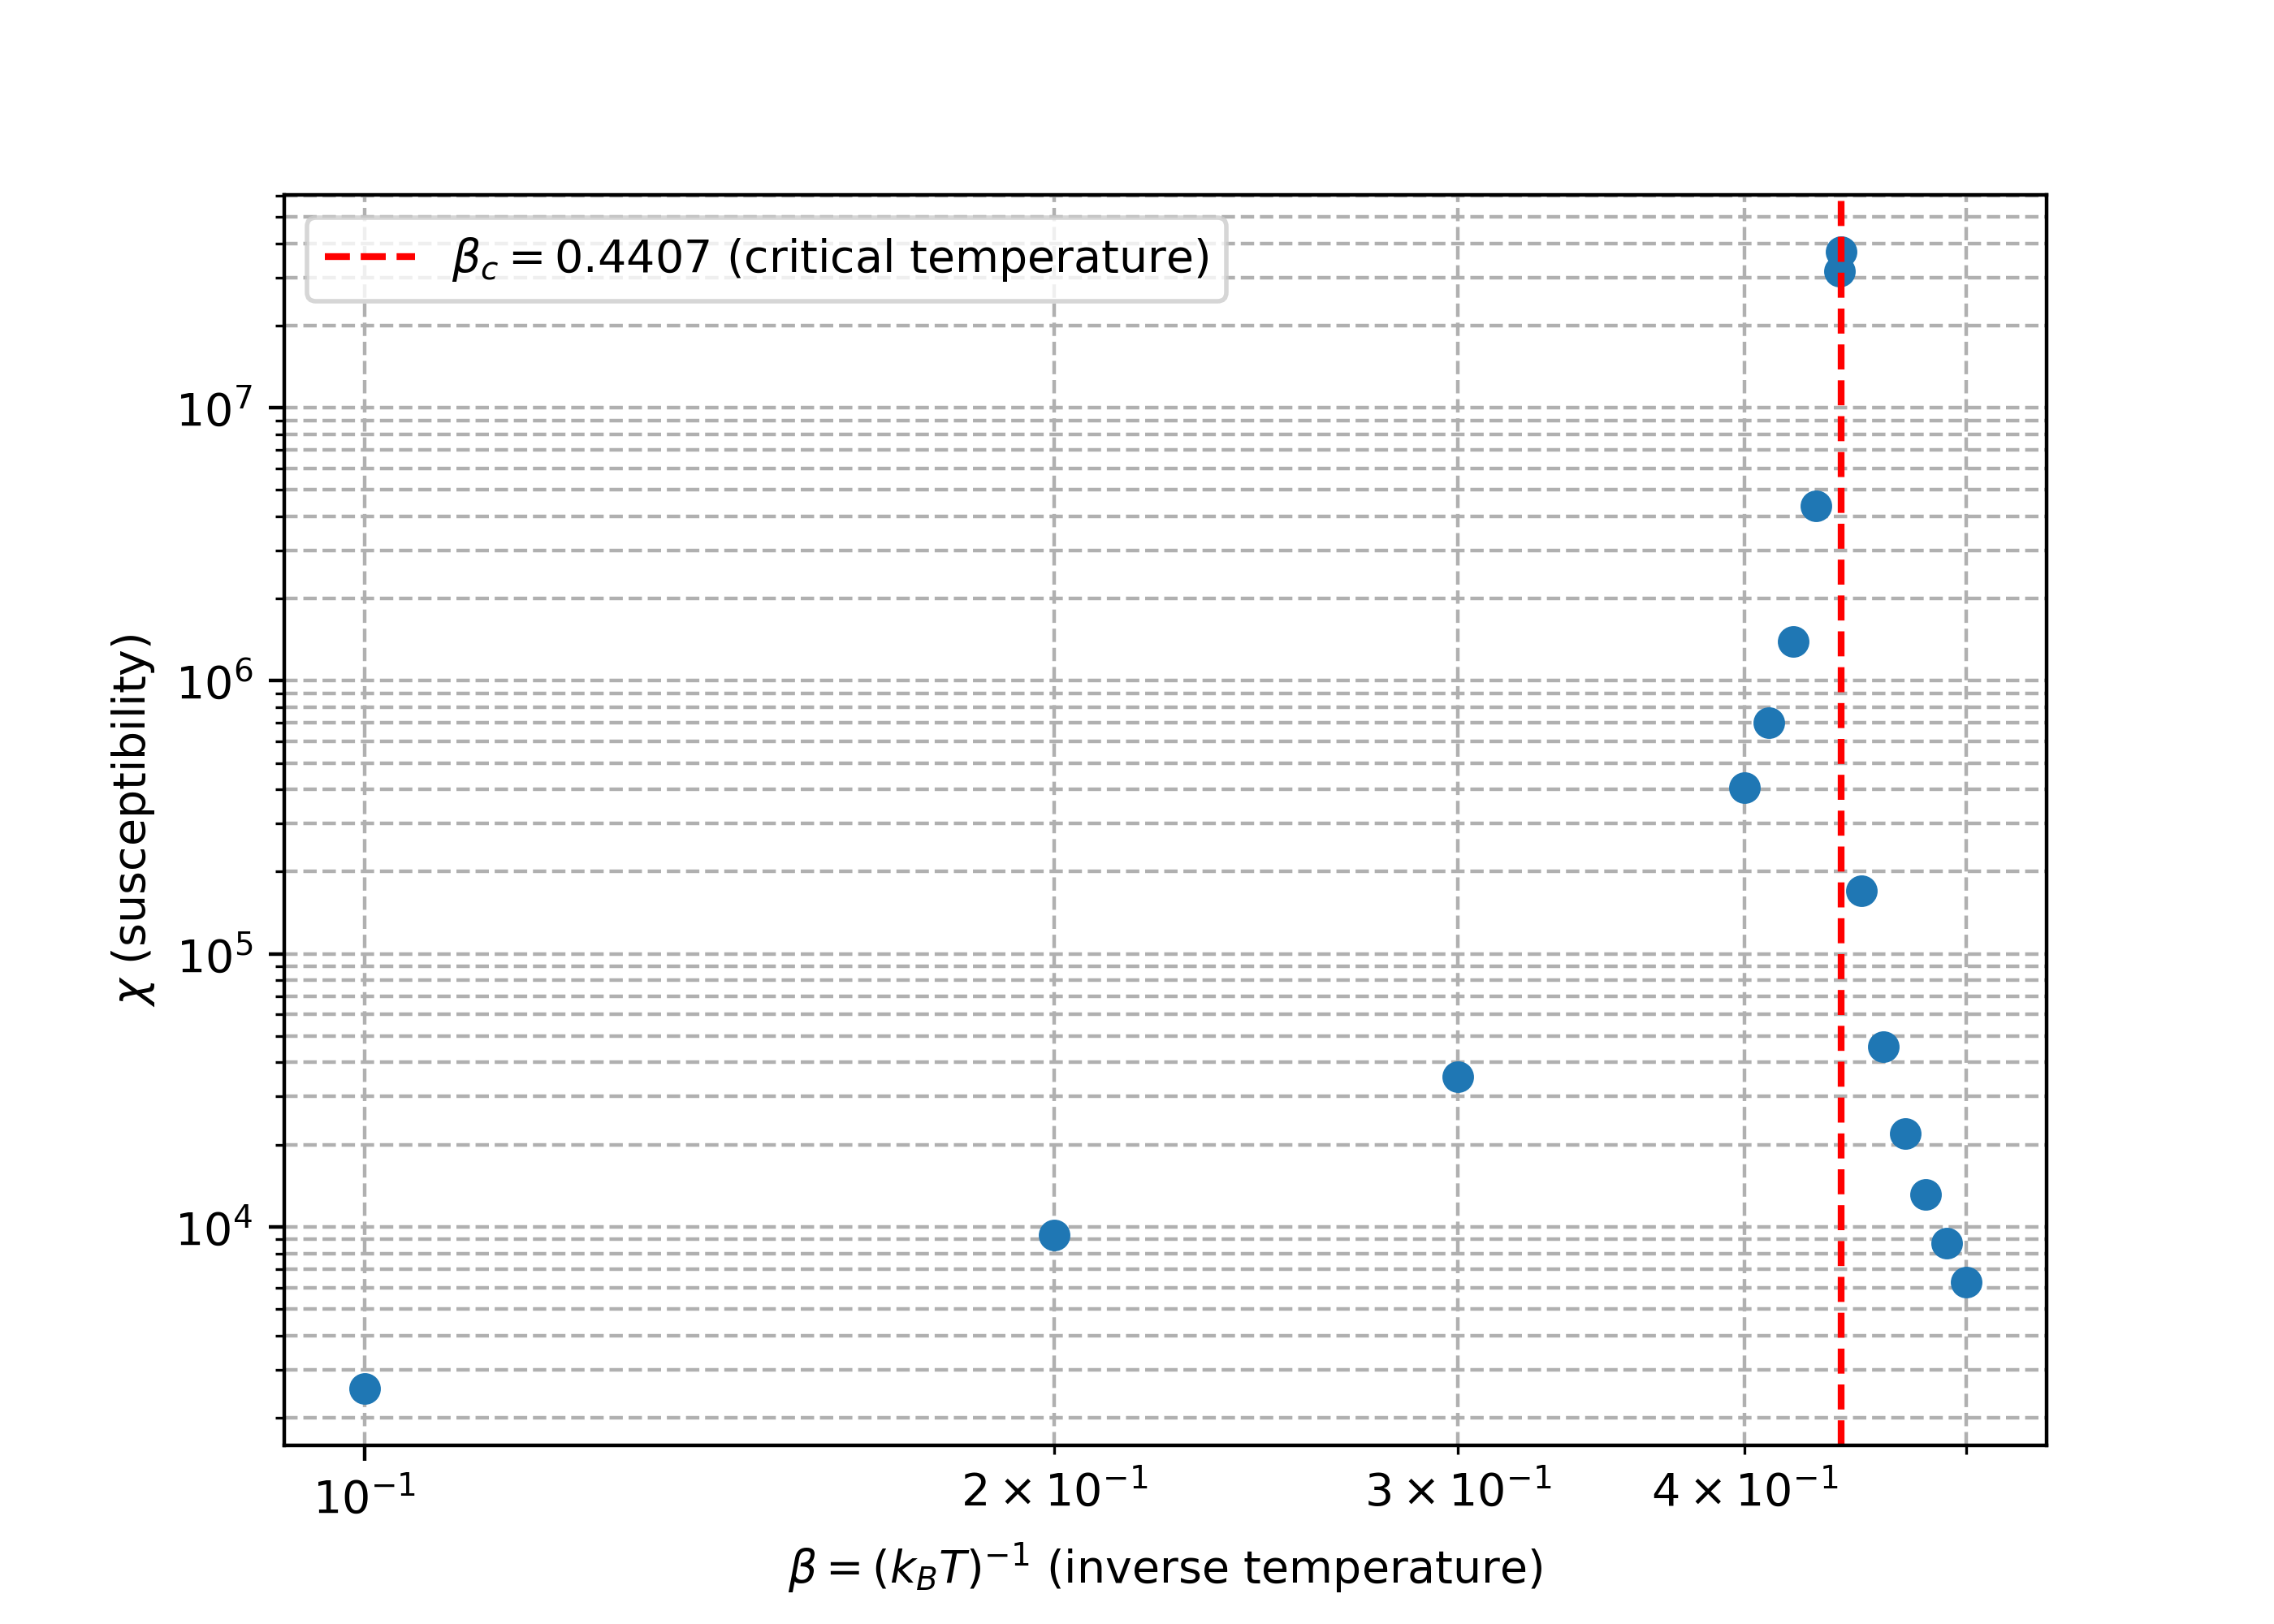
\includegraphics[width = 0.6 \textwidth]{../plots/metropolis_susc_vs_beta_loglog.png}
    \caption[Susceptibility versus $\beta$ using Metropolis updates]{Susceptibility versus inverse temperature $\beta$ using Metropolis updates. Points show the equilibrium susceptibility computed via fluctuation-dissipation theorem.}
\end{figure}

\begin{figure}[h!]
    \centering
    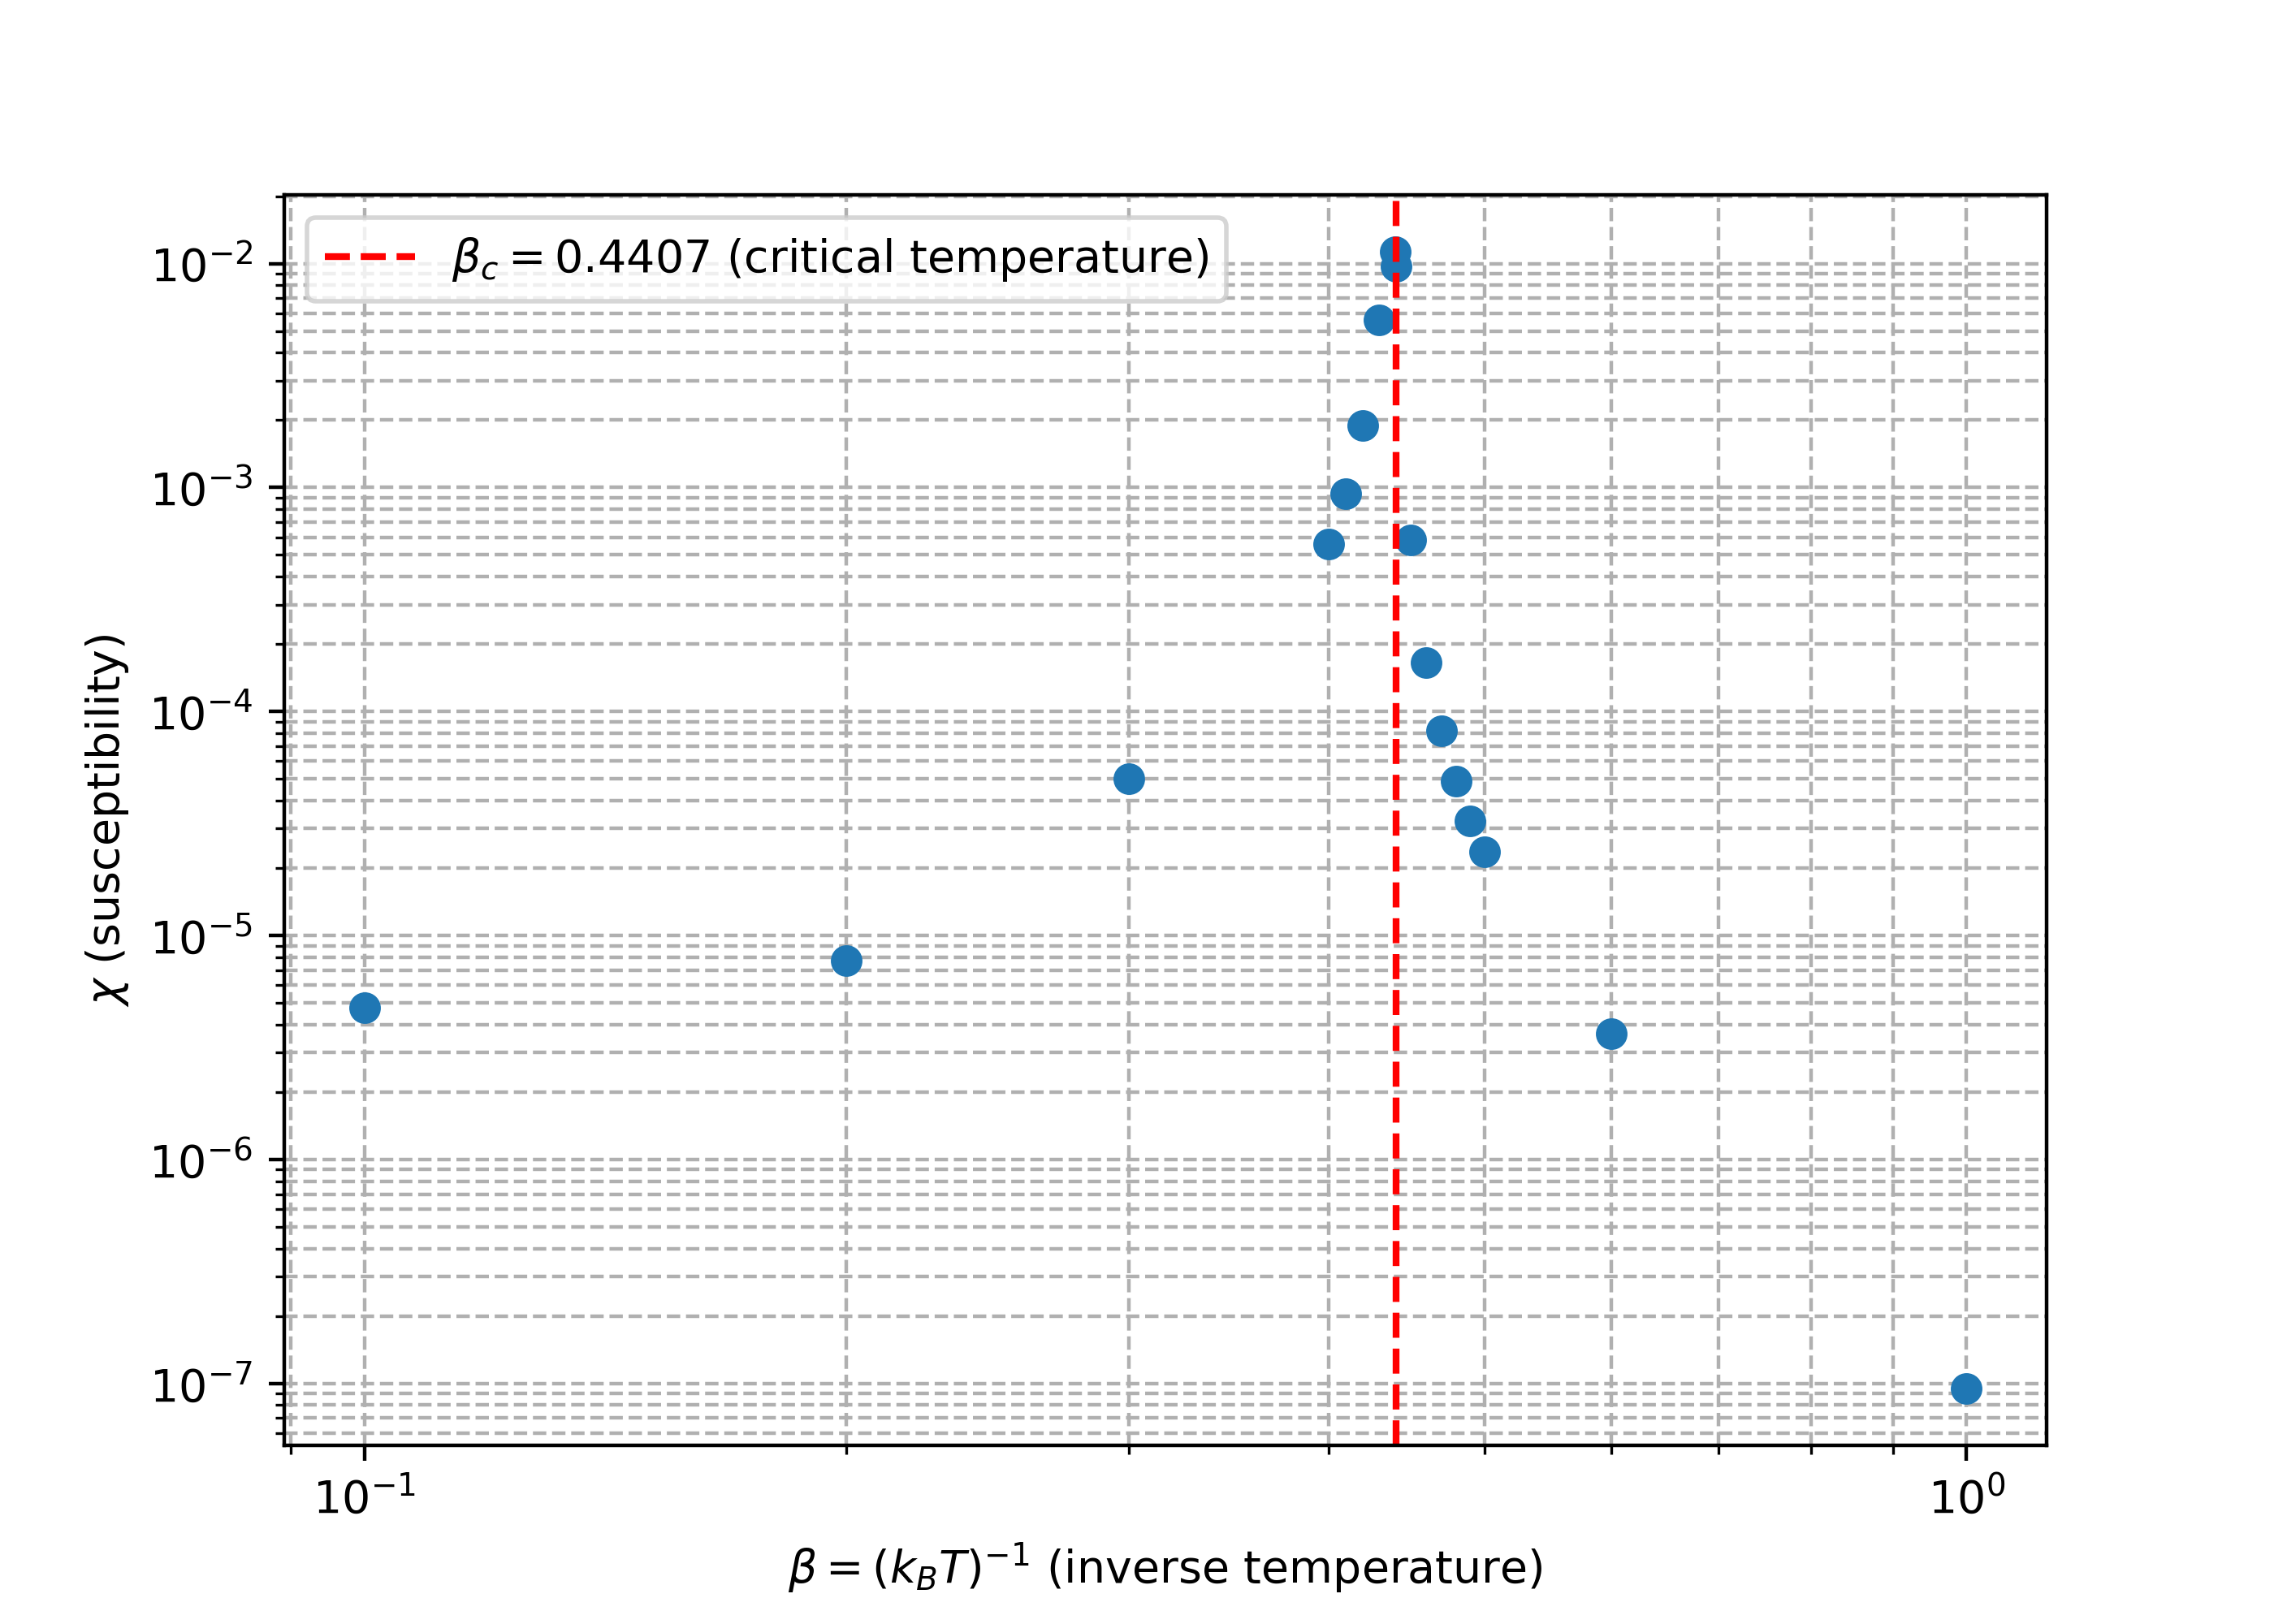
\includegraphics[width = 0.6 \textwidth]{../plots/wolff_susc_vs_beta_loglog.png}
    \caption[Susceptibility versus $\beta$ using Wolff updates]{Susceptibility versus inverse temperature $\beta$ using Wolff updates. Points show the equilibrium susceptibility computed via fluctuation-dissipation theorem.}
\end{figure}

Susceptibility plots exhibit clear peaks near $T_c$ for both algorithms, indicating critical fluctuations as expected.


\subsection{Autocorrelation Behavior}
- Show sample autocorrelation functions for Metropolis and Wolff updates.

- Discuss qualitative differences: slow decay for Metropolis near \(T_c\), fast for Wolff.

\subsection{Divergence near Criticality}
- Plot autocorrelation time \(\tau(T)\) vs. \(|T - T_c|\).

- Fit \(\tau \sim |T - T_c|^{-z\nu}\) or equivalently \(\tau \sim L^{z}\) at \(T_c\) for finite-size scaling.

- Extract dynamic critical exponents \(z_{\text{Metropolis}}\) and \(z_{\text{Wolff}}\)**.

Expected behavior:


- Metropolis: \(z \approx 2.1\)

- Wolff: \(z \approx 0 \text{–} 0.3\)

\subsection{Comparison of Algorithm Efficiency}

- Compare CPU time per independent sample.

- Discuss how cluster algorithms reduce critical slowing down.

